\documentclass[aspectratio=169]{beamer}
\usetheme{Madrid}
\usecolortheme{default}
\usepackage{tikz}
\usetikzlibrary{calc,shapes,arrows.meta,positioning}

% --- Organization slides (TOC + section dividers) ---
\AtBeginSection[]
{
  \begin{frame}{Outline}
    \tableofcontents[currentsection]
  \end{frame}
}

\title{Lecture 2: Costs and Processing}
\subtitle{Vertical Slices, MVPs, Crawling, Walking, and Running}
\author{University of Chicago}
\date{\today}

\begin{document}

\frame{\titlepage}

% Global outline (matches \section{} titles)
\begin{frame}{Outline}
  \tableofcontents
\end{frame}


\section{Development Methodology}

\begin{frame}{System Thinking: Breaking Down AI Tasks}
\begin{itemize}
    \item Before coding, we need to \textbf{think systematically}:
    \begin{enumerate}
        \item How do we abstract and organize our code?
        \item How do we break tasks into inputs and outputs?
        \item How do we organize these into functions?
    \end{enumerate}
    \item \textbf{Plan before you code}
    \item Break down required tasks, \textit{then} start coding
    \item How do we do this? What does it mean to ``break tasks down"?
\end{itemize}
\end{frame}

\begin{frame}{The Development Process}
\textbf{Three-Step Approach:}
\begin{enumerate}
    \item \textbf{Define a vertical slice}
    \begin{itemize}
        \item What is the minimal end-to-end flow?
        \item Start simple, prove it works
    \end{itemize}
    \vspace{0.2cm}
    \item \textbf{Define the systems (functions) required}
    \begin{itemize}
        \item Know the inputs and outputs of each piece
        \item Simpler is better
    \end{itemize}
    \vspace{0.2cm}
    \item \textbf{Then: Crawl $\rightarrow$ Walk $\rightarrow$ Run}
    \begin{itemize}
        \item Start minimal, add features incrementally
    \end{itemize}
\end{enumerate}
\end{frame}

\begin{frame}{Example Problem: Time Series Analysis}
\textbf{Task}: Run a regression on 25 datasets
\vspace{0.3cm}

\textbf{Context}:
\begin{itemize}
    \item We have data from 25 countries
    \item Each CSV contains education and GDP data over time
    \item We want to run a time series analysis on the relationship
\end{itemize}
\vspace{0.3cm}

\textbf{Question}: How do we break this down?
\end{frame}

\begin{frame}{System Design: Complete Problem}
\begin{center}
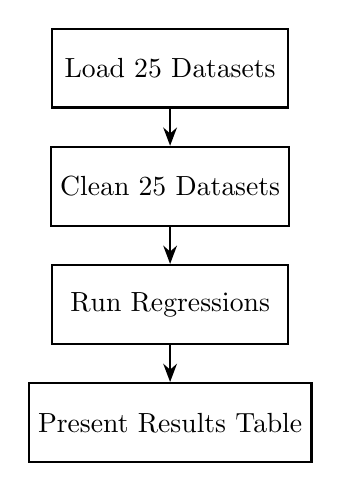
\begin{tikzpicture}[
  box/.style={rectangle, draw, thick, minimum width=3cm, minimum height=1cm, text centered},
  arrow/.style={->, thick, >=Stealth}
]
  \node[box] (load) at (0,0) {Load 25 Datasets};
  \node[box] (clean) at (0,-1.5) {Clean 25 Datasets};
  \node[box] (regress) at (0,-3) {Run Regressions};
  \node[box] (present) at (0,-4.5) {Present Results Table};

  \draw[arrow] (load) -- (clean);
  \draw[arrow] (clean) -- (regress);
  \draw[arrow] (regress) -- (present);
\end{tikzpicture}
\end{center}
\vspace{0.2cm}
This is the \textbf{complete problem}, but where do we start?
\end{frame}

\begin{frame}{Inputs and Outputs: The Missing Piece}
\textbf{For each system component, we need to define:}
\begin{itemize}
    \item \textbf{Load Data}: What format? CSV? Excel? APIs?
    \item \textbf{Clean Data}: What cleaning steps? How do we handle missing values?
    \item \textbf{Run Regression}: What type? Linear? Time series?
    \item \textbf{Present Output}: Table? Graph? JSON? What metrics?
\end{itemize}
\vspace{0.3cm}
\pause
\textbf{This is the complete problem, but we never want to start here!}
\vspace{0.2cm}

We want to start with a \textbf{vertical slice}.
\end{frame}

\begin{frame}{What is a Vertical Slice?}
\textbf{A vertical slice}:
\begin{itemize}
    \item Contains \textbf{everything} needed to go from top to bottom
    \item Works on a \textbf{subset} of inputs
    \item Proves the \textbf{end-to-end flow} works
    \item Is the \textbf{simplest possible} complete solution
\end{itemize}
\vspace{0.3cm}

\textbf{When we build AI systems, we want to start with vertical slices.}
\end{frame}

\begin{frame}{Why Vertical Slices for AI?}
\textbf{AI systems have unique challenges:}
\begin{itemize}
    \item \textbf{Complex}: Many moving parts and dependencies
    \item \textbf{Uncertain failure points}: We aren't sure where things will break
    \item \textbf{Non-deterministic}: Errors appear in unexpected places
    \item \textbf{Iterative prompting}: Prompts need testing and refinement
\end{itemize}
\vspace{0.3cm}

\textbf{With vertical slices}:
\begin{itemize}
    \item We build a viable end-to-end solution that works on a \textbf{subset} of inputs
    \item We discover integration issues \textbf{early}
    \item We can demonstrate \textbf{value quickly}
\end{itemize}
\end{frame}

\begin{frame}{The Opposite: Horizontal Development}
\textbf{Horizontal development} means:
\begin{itemize}
    \item Building for \textbf{all contingencies} at each level
    \item Handling \textbf{every possibility} before moving forward
    \item Creating \textbf{complete infrastructure} before testing end-to-end
\end{itemize}
\vspace{0.3cm}

\textbf{For our regression example}:
\begin{itemize}
    \item Load all 25 datasets with full error handling
    \item Clean all datasets with every edge case covered
    \item Build multiple regression types and robustness checks
    \item Create multiple output formats and visualizations
\end{itemize}
\vspace{0.3cm}

\textbf{Problem}: You spend weeks building infrastructure before knowing if the core idea works!
\end{frame}

\begin{frame}{Vertical Slice: Regression Example}
\begin{center}
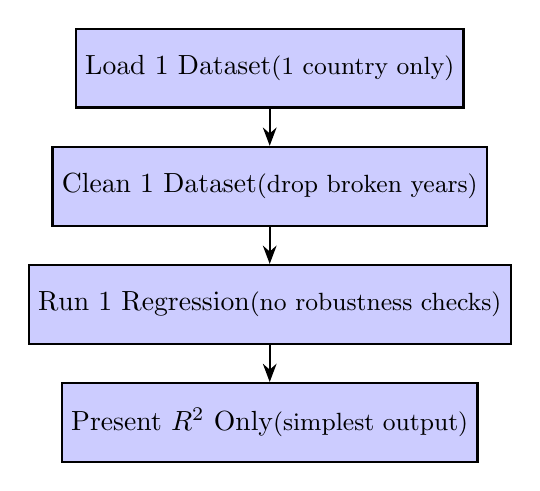
\begin{tikzpicture}[
  box/.style={rectangle, draw, thick, minimum width=4.5cm, minimum height=1cm, text centered},
  arrow/.style={->, thick, >=Stealth}
]
  \node[box, fill=blue!20] (load) at (0,0) {Load 1 Dataset \\ \small (1 country only)};
  \node[box, fill=blue!20] (clean) at (0,-1.5) {Clean 1 Dataset \\ \small (drop broken years)};
  \node[box, fill=blue!20] (regress) at (0,-3) {Run 1 Regression \\ \small (no robustness checks)};
  \node[box, fill=blue!20] (present) at (0,-4.5) {Present $R^2$ Only \\ \small (simplest output)};

  \draw[arrow] (load) -- (clean);
  \draw[arrow] (clean) -- (regress);
  \draw[arrow] (regress) -- (present);
\end{tikzpicture}
\end{center}
\vspace{0.2cm}
\textbf{This proves it works end-to-end with minimal effort!}
\end{frame}

\begin{frame}{Example: Personalized Marketing Emails}
\textbf{Task}: Send AI-generated personalized marketing emails to leads
\vspace{0.3cm}

\textbf{Vertical Slice Approach}:
\begin{itemize}
    \item Load \textbf{one} lead from the database
    \item Generate \textbf{one} email with LLM
    \item Print email to console for manual review
    \item If it looks good, move to next step
\end{itemize}
\vspace{0.3cm}

\textbf{Horizontal Approach} (what NOT to do):
\begin{itemize}
    \item Build complete database integration for all leads
    \item Create email templates for all scenarios
    \item Build full SMTP sending infrastructure
    \item Set up monitoring and analytics before sending anything
\end{itemize}
\end{frame}

\begin{frame}{Principle: Well-Defined Inputs and Outputs}
\begin{itemize}
    \item Each component should have:
    \begin{enumerate}
        \item \textbf{Clear input contract}: What data does it expect? In what format?
        \item \textbf{Clear output contract}: What data does it return? In what format?
        \item \textbf{Single responsibility}: Does one thing well
        \item \textbf{Testability}: Can be tested independently
    \end{enumerate}
    \vspace{0.3cm}
    \item \textbf{Benefits:}
    \begin{itemize}
        \item Easy to understand what each piece does
        \item Easy to test each piece independently
        \item Easy to replace or improve individual pieces
        \item Clear error boundaries
    \end{itemize}
\end{itemize}
\end{frame}

\begin{frame}{Methodology: Crawl, Walk, Run}
\begin{itemize}
    \item \textbf{Crawl}: What is the minimum code to verify it's possible?
    \begin{itemize}
        \item Hardcoded examples
        \item Manual verification
        \item Proof of concept that it can work in \textit{some} instances
    \end{itemize}
    \item \textbf{Walk}: What is the minimum code to verify it works in most cases?
    \begin{itemize}
        \item Handle common edge cases
        \item Basic error handling
        \item Works reliably for typical inputs
    \end{itemize}
    \item \textbf{Run}: What does the full production system look like?
    \begin{itemize}
        \item Comprehensive error handling
        \item Monitoring and logging
        \item Scale and performance optimization
    \end{itemize}
\end{itemize}
\end{frame}

\begin{frame}{Crawl Phase in Detail}
\textbf{Goal}: Prove the concept works at all
\vspace{0.3cm}

\textbf{Characteristics}:
\begin{itemize}
    \item Use \textbf{hardcoded} or sample data
    \item \textbf{No error handling} (let it fail if something breaks)
    \item \textbf{Manual testing} (print statements, visual inspection)
    \item \textbf{Happy path only} (assume everything works)
\end{itemize}
\vspace{0.3cm}

\textbf{Example - Resume Screening}:
\begin{itemize}
    \item Hardcode path to one resume PDF
    \item Extract skills with LLM, print to console
    \item Compare to hardcoded job requirements
    \item Print match score
\end{itemize}
\vspace{0.2cm}
\textbf{If this doesn't work, nothing else matters!}
\end{frame}

\begin{frame}{Building Vertical Slices First}
\begin{itemize}
    \item \textbf{Vertical Slice}: End-to-end functionality for a narrow use case
    \begin{itemize}
        \item Example: Process ONE resume through the entire pipeline
        \item Proves the concept works end-to-end
        \item Surfaces integration issues early
    \end{itemize}
    \vspace{0.3cm}
    \item \textbf{Then Build Horizontally}: Expand capabilities
    \begin{itemize}
        \item Add batch processing
        \item Add error handling
        \item Add more sophisticated matching
        \item Add caching and optimization
    \end{itemize}
\end{itemize}
\end{frame}

\begin{frame}{Key Takeaways: Building with AI}
\begin{enumerate}
\item \textbf{Define the vertical slice} -- what is the minimum thing you can get working?
    \begin{itemize}
        \item Prove end-to-end flow works with simplest case
        \item Identify integration issues early
    \end{itemize}

\item \textbf{Figure out the inputs and outputs}
    \begin{itemize}
        \item Each function needs clear contracts
        \item Simpler is better
    \end{itemize}

\item \textbf{Figure out the pricing}
    \begin{itemize}
        \item Know your costs before scaling
    \end{itemize}

\item \textbf{Expand horizontally after vertical slice works}
    \begin{itemize}
        \item Add batch processing, error handling, features
        \item Don't optimize or add features prematurely
    \end{itemize}

\end{enumerate}
\end{frame}

\section{AI Resume Scoring System}

\begin{frame}{Problem Background}
\begin{itemize}
  \item We have been hired by a company to help with their software developer hiring process
  \item Our goal is to build an AI-assisted resume scoring system
  \item For each resume, we want to score it so that we don't waste time on resumes we are unlikely to hire
  \item We are also cost conscious
\end{itemize}
\end{frame}

\begin{frame}{Brainstorming}
\begin{itemize}
\item How are we going to proceed here?
\item What's our vertical slice?
\item What are the system components?
\item What are the inputs and outputs?
\end{itemize}
\end{frame}

\begin{frame}{Practical Example: Resume Screening System}
\textbf{Phase 1: Vertical Slice (Crawl)}
\begin{enumerate}
    \item Load one resume text
    \item Call LLM to extract skills
    \item Compare to job requirements
    \item Print result
\end{enumerate}
\vspace{0.3cm}
\textbf{Phase 2: Horizontal Expansion (Walk)}
\begin{itemize}
    \item Process all resumes in a directory
    \item Add structured output (JSON, CSV)
    \item Add confidence scores
    \item Handle missing data gracefully
\end{itemize}
\vspace{0.3cm}
\textbf{Phase 3: Production (Run)}
\begin{itemize}
    \item Optimize prompts and costs
    \item Add caching for repeated skills
    \item Add human-in-the-loop review
    \item Monitor accuracy and performance
\end{itemize}
\end{frame}

\begin{frame}{Design Exercise: Break Into Pieces}
Given the task: \textit{``Build a system to screen IT resumes for a job opening''}
\vspace{0.3cm}

\textbf{What are the system pieces?}
\pause
\begin{enumerate}
    \item \textbf{Input}: Resume PDF/text files, job requirements
    \item \textbf{Parse}: Extract text from PDFs
    \item \textbf{Extract}: Identify skills/technologies from resume
    \item \textbf{Match}: Compare skills to job requirements
    \item \textbf{Score}: Calculate fit score
    \item \textbf{Rank}: Sort candidates by score
    \item \textbf{Output}: Ranked list with justifications
\end{enumerate}
\vspace{0.3cm}
\pause
\textbf{Which piece should we build first?}\\
\pause
$\rightarrow$ The middle pieces (Extract + Match), using sample data!
\end{frame}

\end{document}
